\documentclass[12pt]{article}
 
\usepackage[margin=1in]{geometry} 
\usepackage{amsmath,amsthm,amssymb}
\usepackage{graphicx} 
\usepackage{listings}
\usepackage{color}

\definecolor{dkgreen}{rgb}{0,0.6,0}
\definecolor{gray}{rgb}{0.5,0.5,0.5}
\definecolor{mauve}{rgb}{0.58,0,0.82}

\lstset{frame=tb,
  language=Python,
  aboveskip=3mm,
  belowskip=3mm,
  showstringspaces=false,
  columns=flexible,
  basicstyle={\small\ttfamily},
  numbers=none,
  numberstyle=\tiny\color{gray},
  keywordstyle=\color{blue},
  commentstyle=\color{dkgreen},
  stringstyle=\color{mauve},
  breaklines=true,
  breakatwhitespace=true,
  tabsize=2
}



\begin{document}
 
\title{Intro to Cryptography} 
\author{Mark Anderson\\ 
Homework 3}
 
\maketitle
\begin{enumerate}
    \item (25 points) Write Python functions that convert between list and cycle notation for permutations. Test it on 500 random permutations generated in list form, which you will convert to cycle form, and then back to list form to see that you are doing the conversions consistently.
    \begin{lstlisting}
from collections import defaultdict, OrderedDict
from random import randint, shuffle
def cycle_not(L1, val, cyc, final):
    #If the length of the cyc list we've been building up is the same as the length of the original list
    #We are finished and can append the current cyc to the final list
    if len(cyc) == len(L1):
        flat_list = [item for sublist in final for item in sublist]
        final.append(list([item for item in cyc if item not in flat_list]))
        return final[1:]
    #If the value we're looking for is in the cyc sublist already, that means we've reached the end of
    #our cycle, and need to append the first element to the end and close off the cycle
    if L1[val] in cyc:
        val = min([item for item in L1 if item not in cyc])
        val = L1.index(val)
        flat_list = [item for sublist in final for item in sublist]
        final.append(list([item for item in cyc if item not in flat_list]))
        cyc.append(L1[val])
    else:
        #if none of the above are true, then we are still looping through a cycle, and append normally
        cyc.append(L1[val])
    return cycle_not(L1, cyc[-1] - 1, cyc, final)

def list_not(cyc):
    new = defaultdict(int)
    list_not = []

    #We want to loop through the entirety of the cycle notation permutation
    while cyc:
        #Pop off the first 'cycle' from the cycle notation list frmo the left side
        # Ex: (3 2 4 1) (5 6)
        # at iteration 0 sublist = (3 2 4 1) and cyc = (5 6)
        sublist = cyc.pop(0)
        #Loop through the entirety of the sublist
        for i in range(len(sublist)):

            #We start with the first element in the cycle, and add it do a 
            #dictionary corresponding to its value and the next element in the cycle
            # Ex:
            # 3 -> 2
            # 2 -> 4
            # 4 -> 1
            # when we try to index into what comes after 1 in the sublist, we will throw an index error
            #and at that point we add the first item in the sublist to the corresponding element in the dict
            # So for the above permutation, after looping through the entirety of the first sublist our 
            # permutation will look like this
            #   1 2 3 4 5 6
            #   3 4 2 1 _ _
            try:
                new[sublist[i]] = sublist[i + 1]
            except IndexError:
                new[sublist[i]] = sublist[0]

    #This just converts the dictionary into a list in the order of the elements inserted
    for key, val in sorted(new.items()):
        list_not.append(val)
    return list_not

def generate_test_cases():
    numPassed = 0
    numCases = 500
    for i in range(numCases):
        #Generates an ordered list of size [25,100]
        testPerm = list(range(1, randint(25,100)))
        #Shuffles the list generated in order to achieve a "random" permutation
        shuffle(testPerm)

        print("Case %d:" % i)
        print("Original Permutation: %s" % str(testPerm))
        #converts the randomly shuffled list to cycle notation
        cycle = cycle_not(testPerm, 0, [], [[]])
        print("Cycle Notation: %s" % str(cycle))
        #converts the list back into its original notation
        listNot = list_not(cycle)
        print("List Notation: %s" % str(listNot))
        #if value returned from list_not equals the value of the original testPermutation
        # List -> cycle -> list works correctly

        if listNot == testPerm:
            print("Case %d passes" % i)
            numPassed += 1
        else:
            print("Case %d fails" % i)
    print("Passed: %d -- Failed: %d" % (numPassed, numCases - numPassed))

def main():
    generate_test_cases()
if __name__ == "__main__":
    main()
    \end{lstlisting}

    A small sample of the testing suite is given, testing permutations of order 5 to 10, the order of the permutations and the number of cases is shortened just to show a sample, the test suites are programmed for 500 cases.
    \begin{lstlisting}
Case 0:
Original Permutation: [3, 2, 1, 4]
Cycle Notation: [[3, 1], [2], [4]]
List Notation: [3, 2, 1, 4]
Case 0 passes
Case 1:
Original Permutation: [5, 2, 4, 6, 3, 7, 1, 9, 8]
Cycle Notation: [[5, 3, 4, 6, 7, 1], [2], [8, 9]]
List Notation: [5, 2, 4, 6, 3, 7, 1, 9, 8]
Case 1 passes
Case 2:
Original Permutation: [7, 1, 4, 3, 6, 2, 5]
Cycle Notation: [[7, 5, 6, 2, 1], [3, 4]]
List Notation: [7, 1, 4, 3, 6, 2, 5]
Case 2 passes
Case 3:
Original Permutation: [1, 2, 3, 4]
Cycle Notation: [[1], [2], [3], [4]]
List Notation: [1, 2, 3, 4]
Case 3 passes
Case 4:
Original Permutation: [7, 1, 3, 5, 6, 2, 4]
Cycle Notation: [[7, 4, 5, 6, 2, 1], [3]]
List Notation: [7, 1, 3, 5, 6, 2, 4]
Case 4 passes
Passed: 5 -- Failed: 0
    \end{lstlisting}
    
  \item Extend the permutation-list multiplication program to include multiplication of cycles.
    \begin{lstlisting}
#Given a permutation in cycle notation, and a value, this function will return the next value in the list
#If the valuee we're looking for is the last value in the list, we return the first element because
#we have found the end of the cycle
def findNext(perm, val):
    for subl in perm:
        for i in range(0, len(subl)):
            #We have found the position in the list that corresponds to the value we're looking for
            if subl[i] == val:
                try:
                    #as stated above, if there is an element that is after the value (meaning we are still cycling)
                    #we return that value
                    val = subl[i + 1]
                except IndexError:
                    #If we are at the last position in the list, we return the first element in the list, because
                    #we have reached the end of the cycle, and the next element is the beginning
                    val = subl[0]

                return val
    return 0

def cycle_mult(P1, P2):
    mult = []
    submult = []
    #A flattened list for easier searching and removal of already processed values
    flat_list = [item for sublist in P2 for item in sublist]
    nextVal = flat_list[0]

    #While the list is not empty (meaning we still have values left to multiply)
    while flat_list:
        #The value to search for in the LHS is the next value in the cycle from the RHS
        val = findNext(P1, nextVal)
        #If the value is already in the sublist we've been building up, we've reached the end of
        #the given cycle, and append it to the final list
        if val in submult:
            mult.append(submult)
            #the new sublist will start with the minimum remaining value
            submult = [min(flat_list)]
        else:
            #none of the above wer met, so we append normally
            submult.append(val)

        #Choose the next value to process based on what comes next in the cycle
        nextVal = findNext(P2, submult[-1])
        #Remove the element we just processed, as to not loop over again
        flat_list.remove(submult[-1])

    mult.append(submult)
    return mult



def cyc_mult_test():
    numCases = 500
    numPassed = 0
    for i in range(numCases):
        length = randint(5,100)
        perm_one = list(range(1,length))
        perm_two = list(range(1,length))
        shuffle(perm_one)
        shuffle(perm_two)
        perm_one_cycle = cycle_not(perm_one, 0, [], [[]])
        perm_two_cycle = cycle_not(perm_two, 0, [], [[]])
        print("Cycle_one: %s" % str(perm_one_cycle))
        print("Cycle_two: %s" % str(perm_two_cycle))
        cycle_m = cycle_mult(perm_one_cycle, perm_two_cycle)
        print("Cycle Multiplication Result: %s" % str(cycle_m))
        list_m = permMult(perm_one, perm_two)
        print("Multiplication Result of given Multiplication Function: %s" % str(list_m))
        cycle_m_list = list_not(cycle_m)
        print("Converted List notation of My Function: %s" % str(cycle_m_list))

        if cycle_m_list == list_m:
            print("Case %d PASSES")
            numPassed += 1
        else:
            print("Case %d FAILS")

    print("Passed: %d -- Failed: %d" % (numPassed, numCases - numPassed))

def permMult(P1, P2):
    if (0 in P1) != (0 in P2):
        return "Base error"
    if len(P1) != len(P2):
        return "Len error"
    if 0 not in P1:
        base = 1
        P1 = [0] + P1
        P2 = [0] + P2
    else:
        base = 0
    pout = [ P1[P2[i]] for i in range(len(P1))]
    return pout[base:]

def main():
    cyc_mult_test()

if __name__ == "__main__":
    main()
    \end{lstlisting}
  
    A small sample of the testing suite is given, testing permutations of order 5 to 10, the order of the permutations and the number of cases is shortened just to show a sample, the test suites are programmed for 500 cases.
    \begin{lstlisting}
Case 0:
Cycle_one: [[8, 6, 2, 5, 1], [3], [4, 7]]
Cycle_two: [[8, 4, 5, 6, 7, 2, 3, 1]]
Cycle Multiplication Result: [[6, 4, 1], [2, 3, 8, 7, 5]]
Multiplication Result of given Multiplication Function: [6, 3, 8, 1, 2, 4, 5, 7]
Converted List notation of My Function: [6, 3, 8, 1, 2, 4, 5, 7]
Case 0 PASSES

Case 1:
Cycle_one: [[3, 5, 4, 1], [2]]
Cycle_two: [[2, 4, 5, 1], [3]]
Cycle Multiplication Result: [[2, 1], [3, 5], [4]]
Multiplication Result of given Multiplication Function: [2, 1, 5, 4, 3]
Converted List notation of My Function: [2, 1, 5, 4, 3]
Case 1 PASSES

Case 2:
Cycle_one: [[2, 4, 6, 3, 1], [5]]
Cycle_two: [[1], [2, 6, 4], [3], [5]]
Cycle Multiplication Result: [[2, 3, 1], [4], [5], [6]]
Multiplication Result of given Multiplication Function: [2, 3, 1, 4, 5, 6]
Converted List notation of My Function: [2, 3, 1, 4, 5, 6]
Case 2 PASSES

Case 3:
Cycle_one: [[4, 5, 3, 7, 2, 9, 6, 8, 1]]
Cycle_two: [[4, 6, 5, 3, 2, 9, 8, 1], [7]]
Cycle Multiplication Result: [[5, 7, 2, 6, 3, 9, 1], [4, 8]]
Multiplication Result of given Multiplication Function: [5, 6, 9, 8, 7, 3, 2, 4, 1]
Converted List notation of My Function: [5, 6, 9, 8, 7, 3, 2, 4, 1]
Case 3 PASSES

Case 4:
Cycle_one: [[2, 3, 4, 1]]
Cycle_two: [[1], [2], [3], [4]]
Cycle Multiplication Result: [[2, 3, 4, 1]]
Multiplication Result of given Multiplication Function: [2, 3, 4, 1]
Converted List notation of My Function: [2, 3, 4, 1]
Case 4 PASSES

Passed: 5 -- Failed: 0
    \end{lstlisting}
  \item Suppose you have two coins: a fair coin and a biased coin that always comes up heads. Suppose you pick one of the coins at random and toss it k times and it produces k heads. Derive a formula depending on k for the probability that you have chosen the biased coin.
  \par
  The final probability that we are looking for in this question is $ P(B | H_1 \cap H_2 \cap ... \cap H_k )$ where $P(B)$ is the probability of the biased coin being chosen, and $P(H_k)$ is the probability of K heads being flipped.  In english, we are looking for the probability that given K flips resulting in K heads, that the coin is the biased coin.\par
  P(B) = 0.5 (1 / number of coins)\par
  P(A) = 0.5 (A being unbiased, B being biased) \par
  $P(H)$ = $ P(H | A) \cup P(H | B)$\par
  $P(H | B) = 1$ and $P {H | A} = \frac{1}{2}$\par
  $P(H_k | B) = \frac{1^k}{2} $ and $P(H_k | A) = \frac{\frac{1}{2}^k}{2} $

  \item Category Theory
    \begin{enumerate}
      \item Prove that a function in the category of sets is an epimorphism iff it is surjective.
        A function $f: A \rightarrow B$ is an epimorphism iff $\forall g_1, g_2 : B \rightarrow C $ $ g_1 * f = g_2 * f \rightarrow g_1 = g_2 $
        \par
        Let $f: A \rightarrow B $ be surjective and let $ g_1, g_2 : B \rightarrow C $ we must prove $ g_1 * f = g_2 * f \rightarrow g_1 = g_2 $
        \par
        Prove that the value of sin(0) = 1 
        \begin{flalign*}
          $ \exists \theta \in \mathbb{Z}$

          g_1*f &= g_2*f \tag{f being surjective must contain a mapping back to the id} &\\
          (g_1 * f) * f^{-1} &= (g_2 * f) * f^{-1} &\\
          g_1 * f * f^{-1} &= g_2 * f * f^{-1} &\\
          g_1 * (f * f^{-1}) &= g_2 * (f * f^{-1}) \tag{$f * f^{-1} = id_B$} &\\
          g_1 * (id_b) &= g_2  * (id_b) &\\
          g_1 &= g_2
        \end{flalign*}
        Proof epimorphism $ \rightarrow $ surjective
        Suppose that $ f:A \rightarrow B $ is not surjective.  Then there may exist $ x \in B $ s.t. $ x \notin image(f) $ this allows the possibility that if $ g_1,g_2:B \rightarrow C$ and with the chosen element x $ g_1(x) \ne g_2(x)$ which violates the morphism, which means it must be surjective.
      \item Prove that a function in the category of sets is a bimporphism iff it is bijective.
        For a function to be a bimorphism, it must be an epimorphism, and a monomorphism.  We know that $f: A \rightarrow B$, $g_1,g_2:B \rightarrow C$, $g_1 * f = g_2 * f \rightarrow g_1 = g_2$ because we proved this above, and for a function to be bijective, it must be surjective.  Since this is a Category of sets, we know that the operation on these two categories must be associative thus we can write a bimorphism as such $ f * (g_1 * f) = f * (g_2 * f) $.  So to prove that the function is a bimorhism, we must prove that it is injective/monomorhism.
        \par
        Proof injective $ \rightarrow $ monomorphism:
        Let $f:A \rightarrow B $ be injective and let $ g_1, g_2:B \rightarrow C $
        \begin{flalign*}
          f * g_1 &= f * g_2 &\\
          f * (g_1(x)) &= f * (g_2(x)) \forall x \in C   
        \end{flalign*}
        Since f is injective, $g_1(x)$ must equal $g_2(x)$ (one-to-one), therefore it is a monomorphism
        \par
        Proof monomorphism $ \rightarrow $ injective:
        Suppose that f is not injective, $ \exists x,y \in A $ s.t. $ x \ne y $ and $f(x) = f(y)$, let $g_1: B \rightarrow A = g_1(1) = x $ and $ g_2: B \rightarrow A = g_2(1) = y $ clearly $ x \ne y $ so f must be injective.  With all of the above conditions true, if a function is bijective, it must be a bimorphism.
      \item Prove that in the category of graphs, the identity function on vertices is the identity morphism.
      \item Describe what a natural functor from the category of graphs to the category of digraphs looks like.\par
      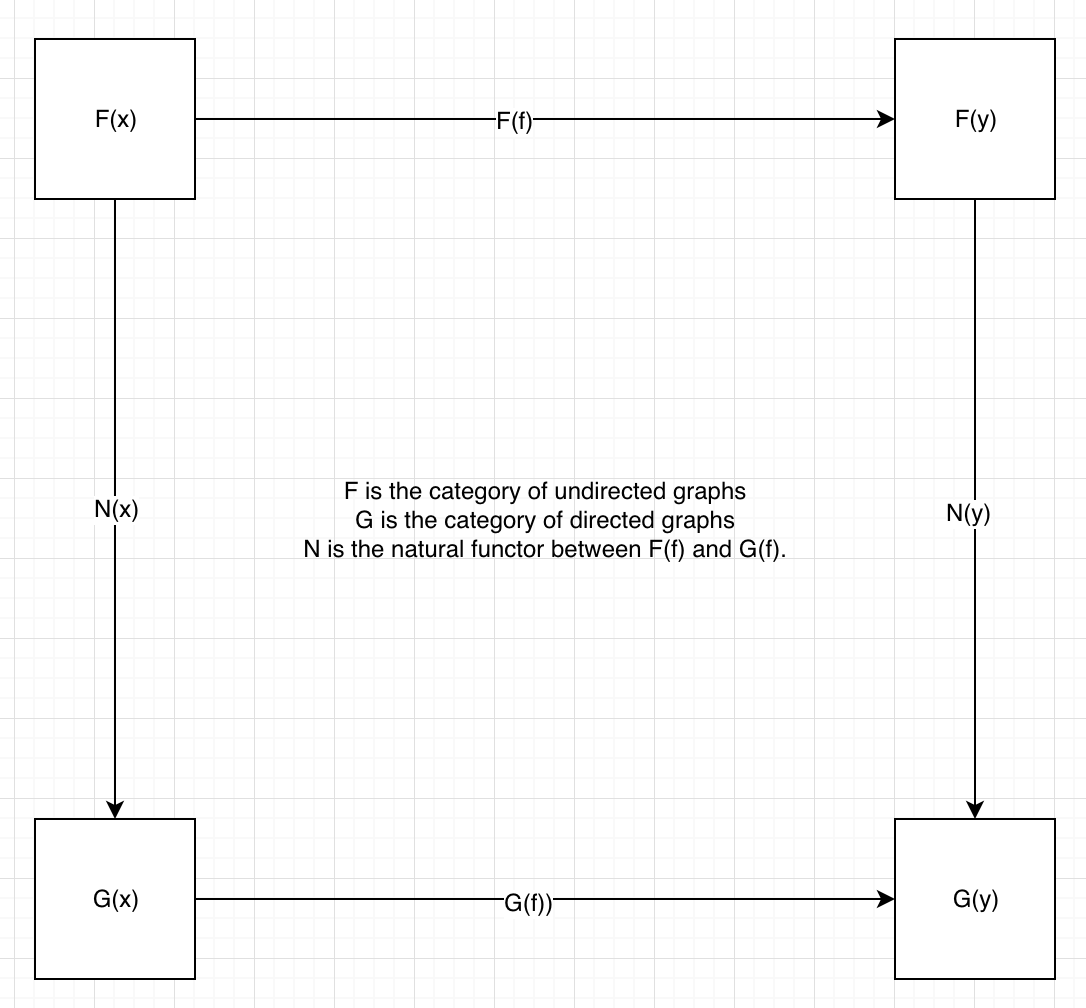
\includegraphics[width=0.55\textheight,height=\textheight,keepaspectratio]{cat.png}
      \par
        The function f maps the vertices in the respective graphs together, s.t f will only map vertices if there is an edge connecting them, and in the case of digraphs, a directed edge connecting them.  The natural functor between these two functions $ F(f), G(f) $ is denoted by $ n: F(f) \rightarrow G(f) $ connects these two functions such that it preserves the structure of the original category.  If we take the natural functor from graphs to digraphs, then the natural functor will take the vertices in the digraphs, and add edges in both directions for all vertices. 
    \end{enumerate}

  \item Describe in detail all groups (up to isomorphism) of order 1,2,....,7.  Which of these groups can be found in $S_4$?
  \item Quadratic Residue - Let p be a prime.
    \begin{enumerate}
      \item Let r and s be quadratic residues mod p.  Prove that rs is a quadratic residue of p.
      \item Let r be a quadratic residue mod p and s a quadratic non-residue mod p.  Prove that rs is a quadratic non-residue of p.
      \item Let r and s be quadratic non-residues mod p.  Prove that rs is a quadratic residue mod p.
    \end{enumerate}
\end{enumerate}



\end{document}
